\documentclass{article}
\usepackage[utf8]{inputenc}
\usepackage{url}
\usepackage{graphicx}
\graphicspath{ {./} }


\title{Automatisation du prétraitement de photographies de portraits de mandrills}
\author{Maxime Boucher}
\date{Compte rendu 2}

\begin{document}

\maketitle

Depuis la dernière fois, j'ai travaillé sur la matrice de confusion, le graphe ROC et commencer à comparer deux trois choses.\\

Nous démarrons avec un transfer learning par VGG16/ImageNet suivi de deux couches complètements connectés, par enfin une couche softmax (probabilités).

Nous obtenons sur 10 epochs un rappel à 0.8 pour les 2 classes les plus représentés (FaceQual3/2) et 0.65 pour les autres (FaceQual0/1). Cela veut donc dire qu'une proportion correcte initiale d'échantillons est correctement classé.

\begin{center}
    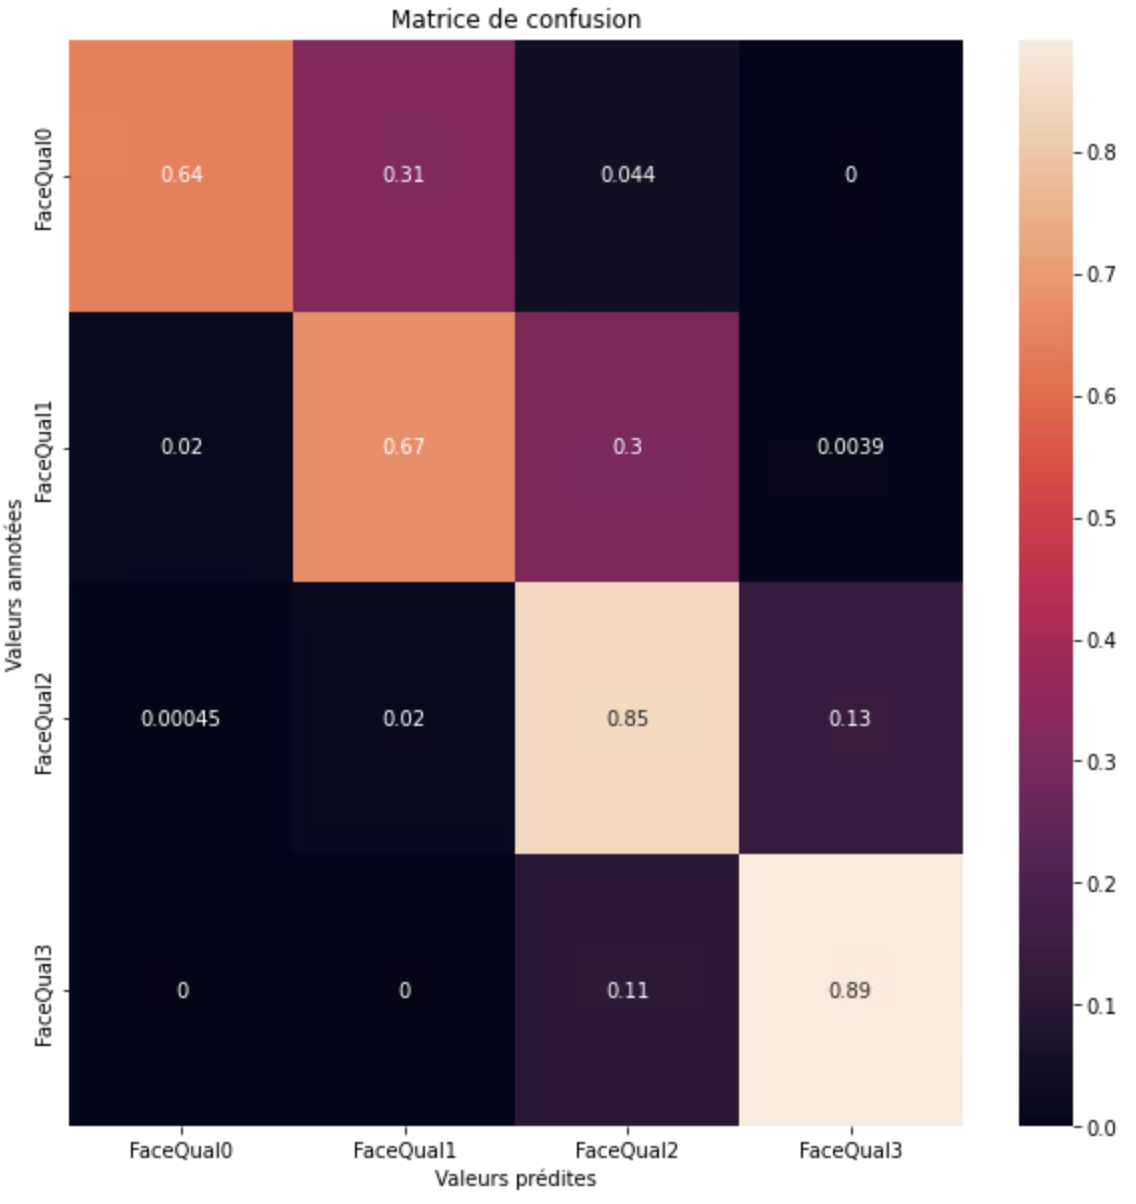
\includegraphics[width=150]{imgs/qualité/cr2/vgg16_000_confusion.png}
    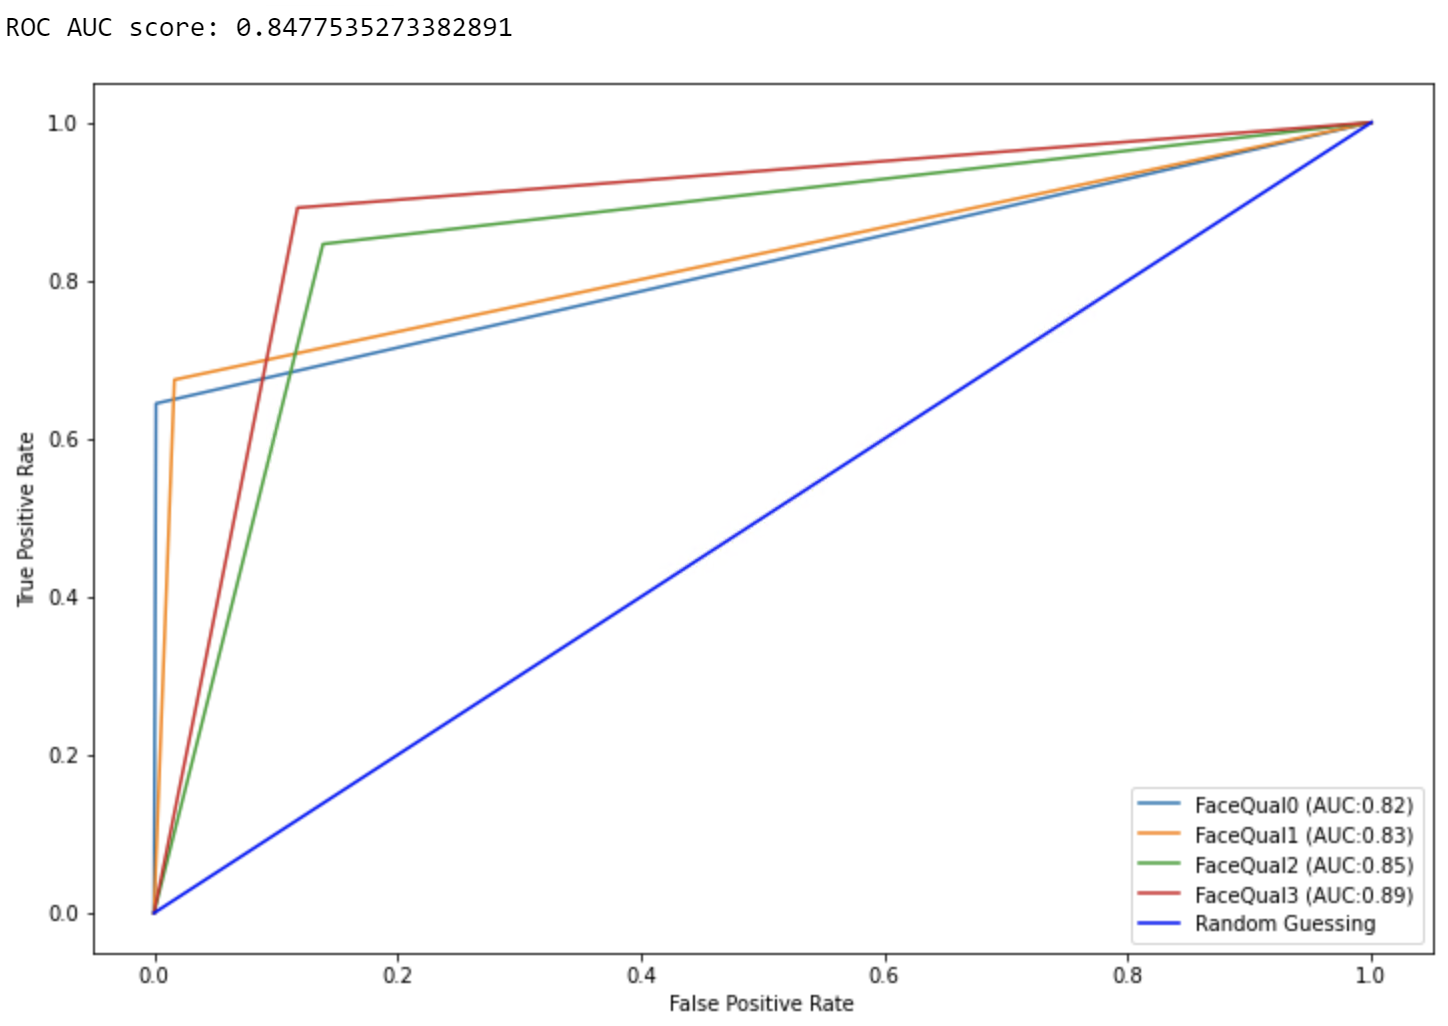
\includegraphics[width=150]{imgs/qualité/cr2/vgg16_000_roc.png}
\end{center}

Pour améliorer la situation, problématique sûrement à cause du déséquilibre des données, nous pouvons essayer d'abord la pondération des classes. Cela permet en effet d'améliorer largement le résultat de la classe la plus sous représentée (FaceQual0), avec un poids d'importance de 17. Seulement, une partie de l'apprentissage est troublée, d'une part car la classe FaceQual1 est partiellement confondue par la classe FaceQual0 et également du fait que beaucoup d'échantillons FaceQual2 sont classés en FaceQual0 (5\% des FaceQual2, représentant une bonne partie sachant que FaceQual2 possède énormément plus d'images).


\begin{center}
    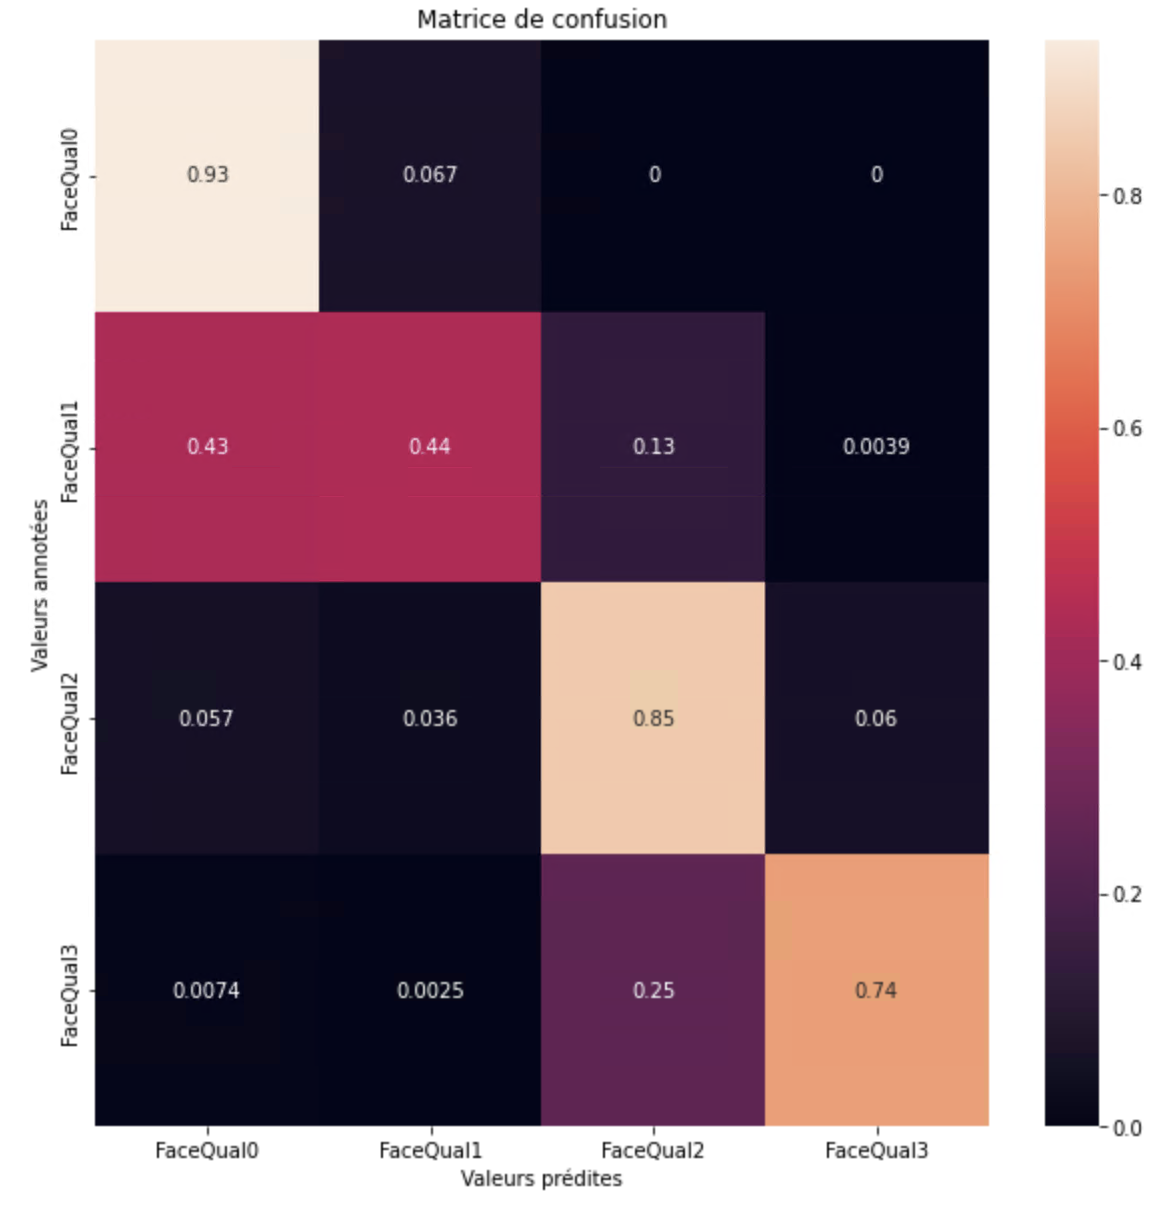
\includegraphics[width=150]{imgs/qualité/cr2/vgg16_010_confusion.png}
    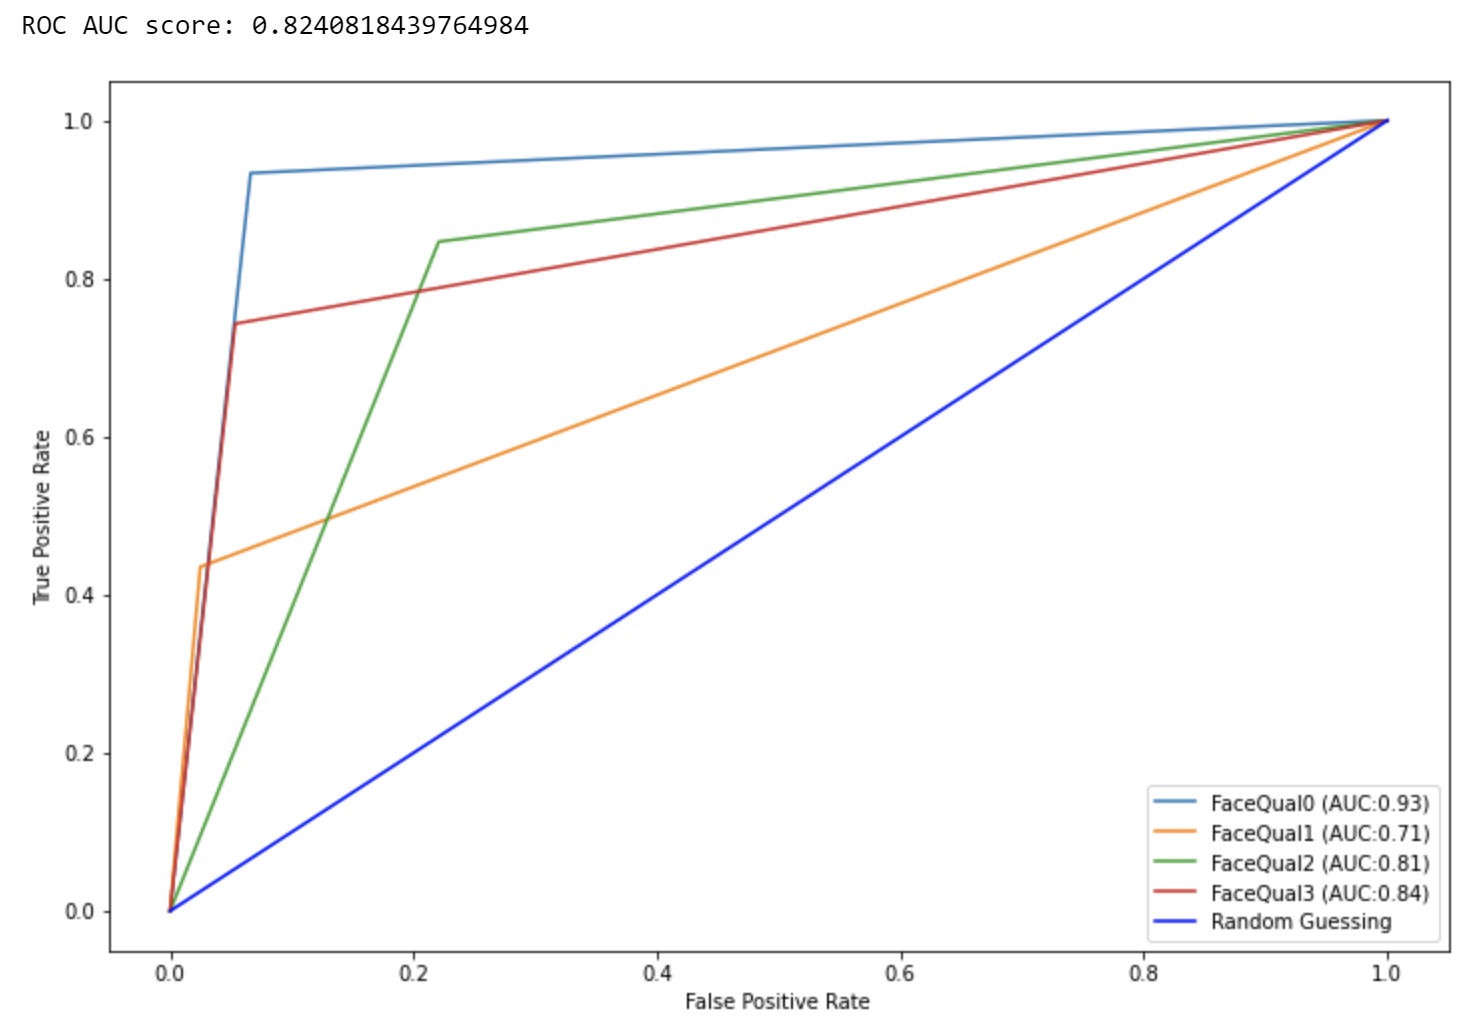
\includegraphics[width=150]{imgs/qualité/cr2/vgg16_010_roc.png}
\end{center}

Une piste est alors d'opérer un oversampling a priori sur la classe FaceQual0 pour avoir des poids de classes plus adéquats (moins grands). \\

Une fois testé, nous trouvons un rappel supérieur à la situation initiale sans cette fois-ci occasionner de dommages collatéraux. Le poids de la classe FaceQual0 après l'oversampling par copie/dégradation des images FaceQual3 est autour de 4, soit 4 fois moins qu'avant oversampling.

\begin{center}
    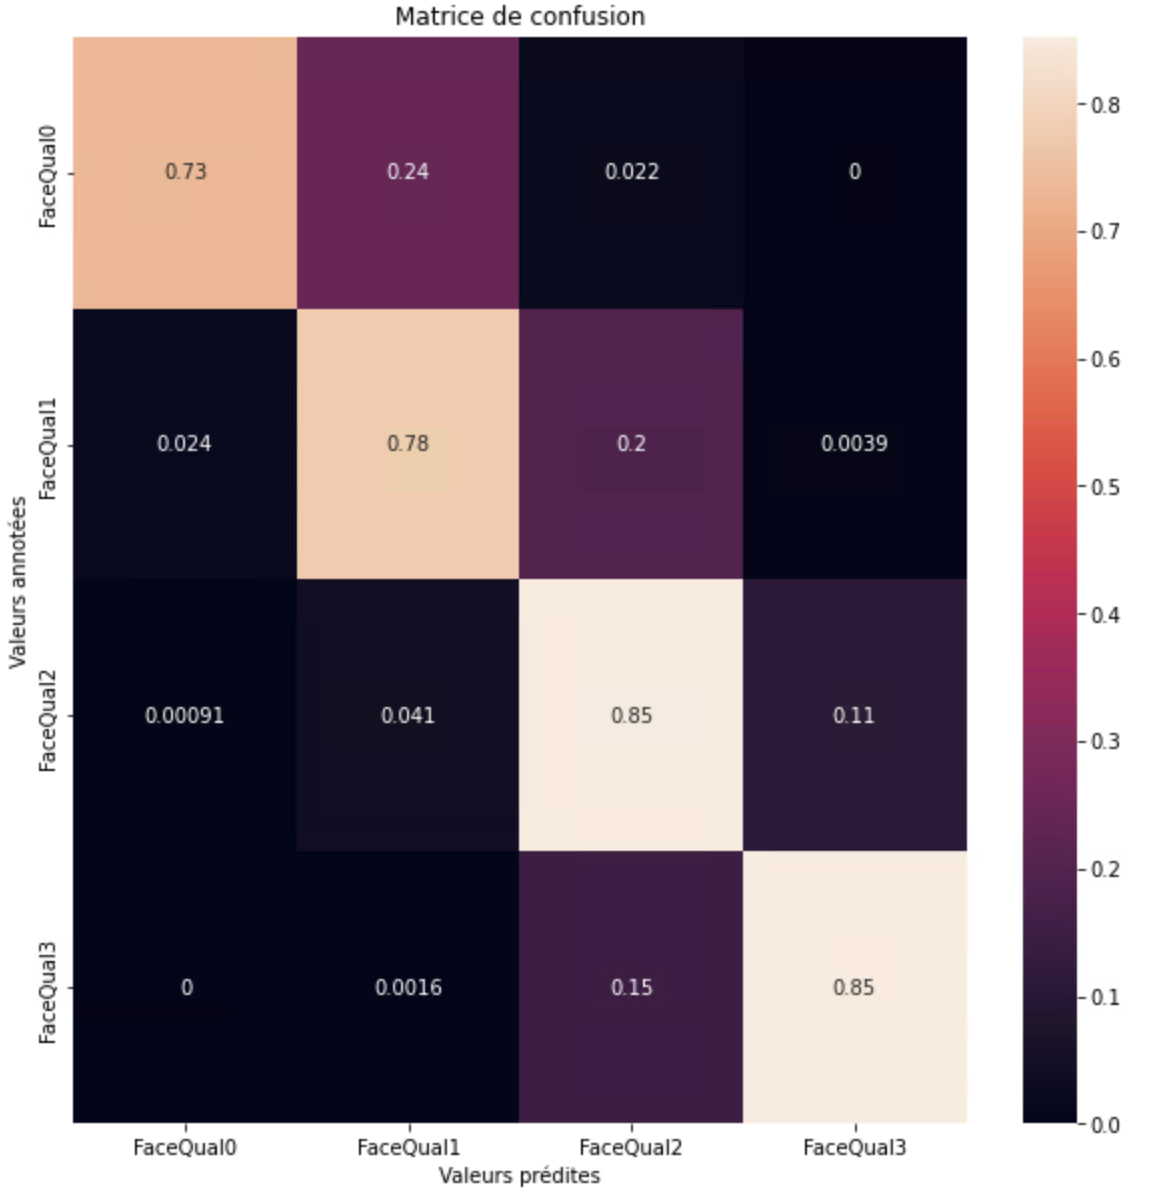
\includegraphics[width=150]{imgs/qualité/cr2/vgg16_011_confusion.png}
    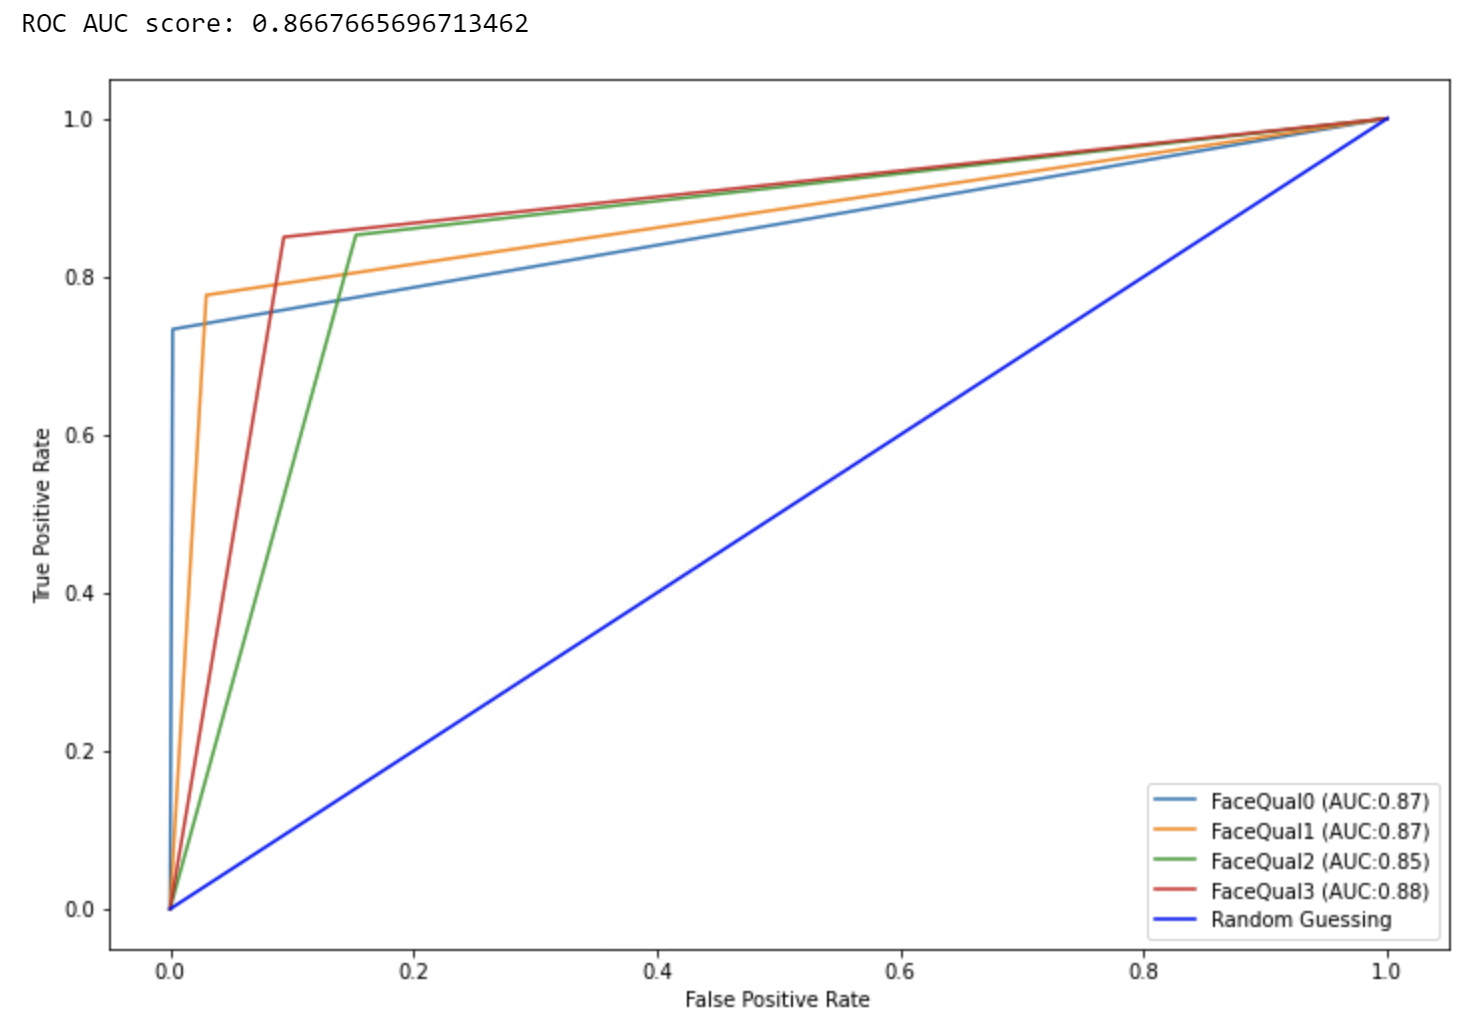
\includegraphics[width=150]{imgs/qualité/cr2/vgg16_011_roc.png}
\end{center}

Avec un peu de fine-tuning par dégel progressif des couches externes de VGG16, nous pouvons obtenir ces derniers résultats. L'enjeu sera dans les prochains jours de trouver les bons paramètres de modifications pour obtenir les meilleurs résultats.


\begin{center}
    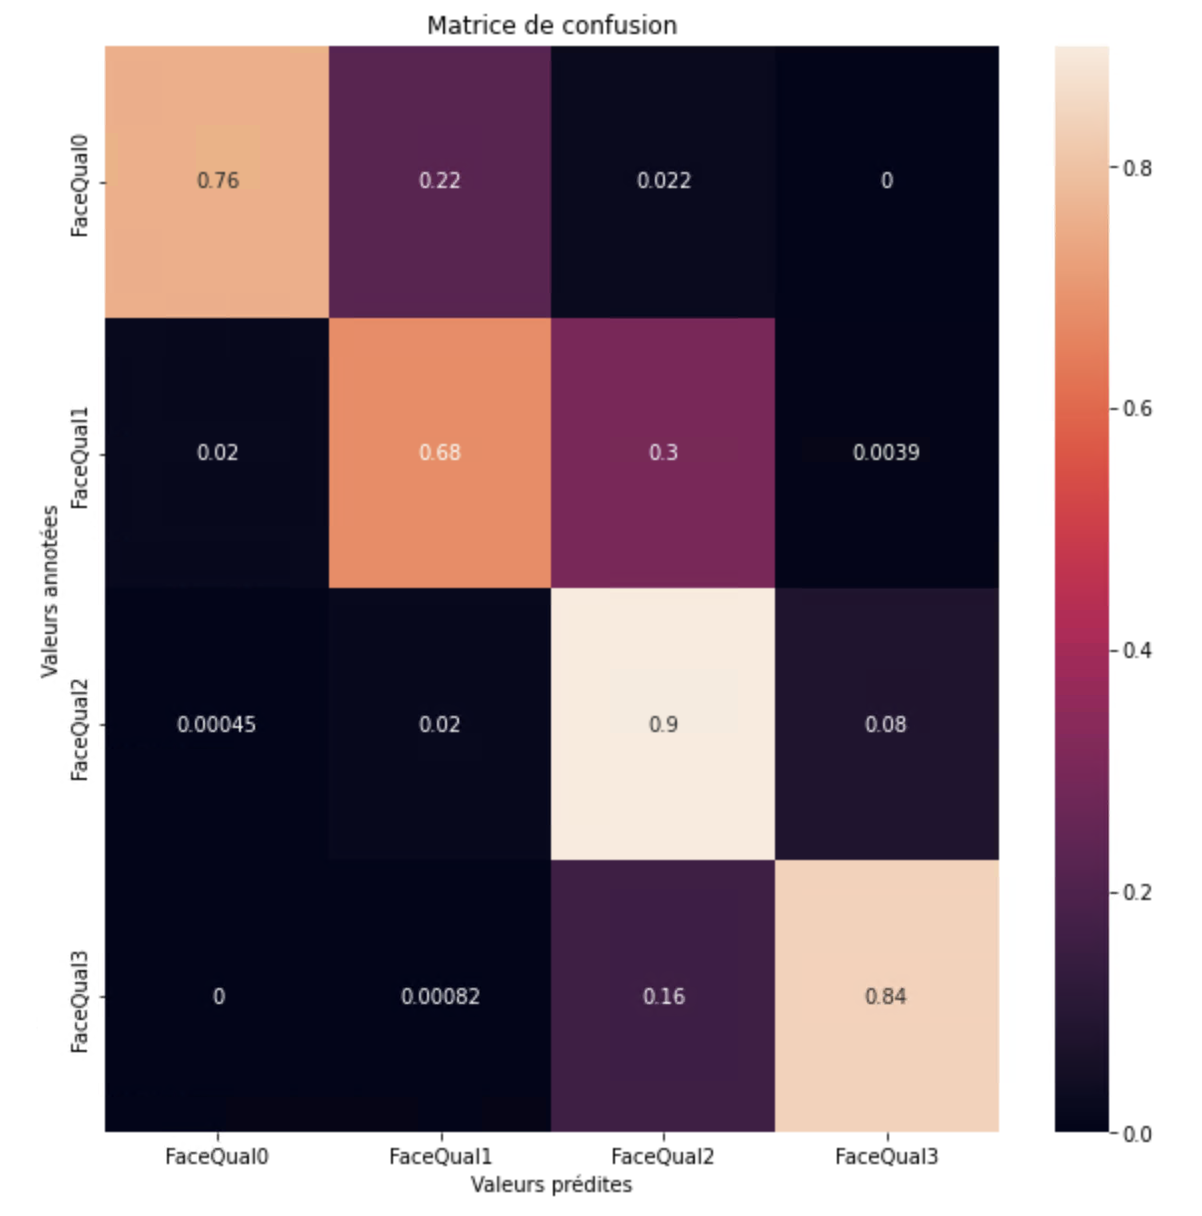
\includegraphics[width=150]{imgs/qualité/cr2/vgg16_111_confusion.png}
    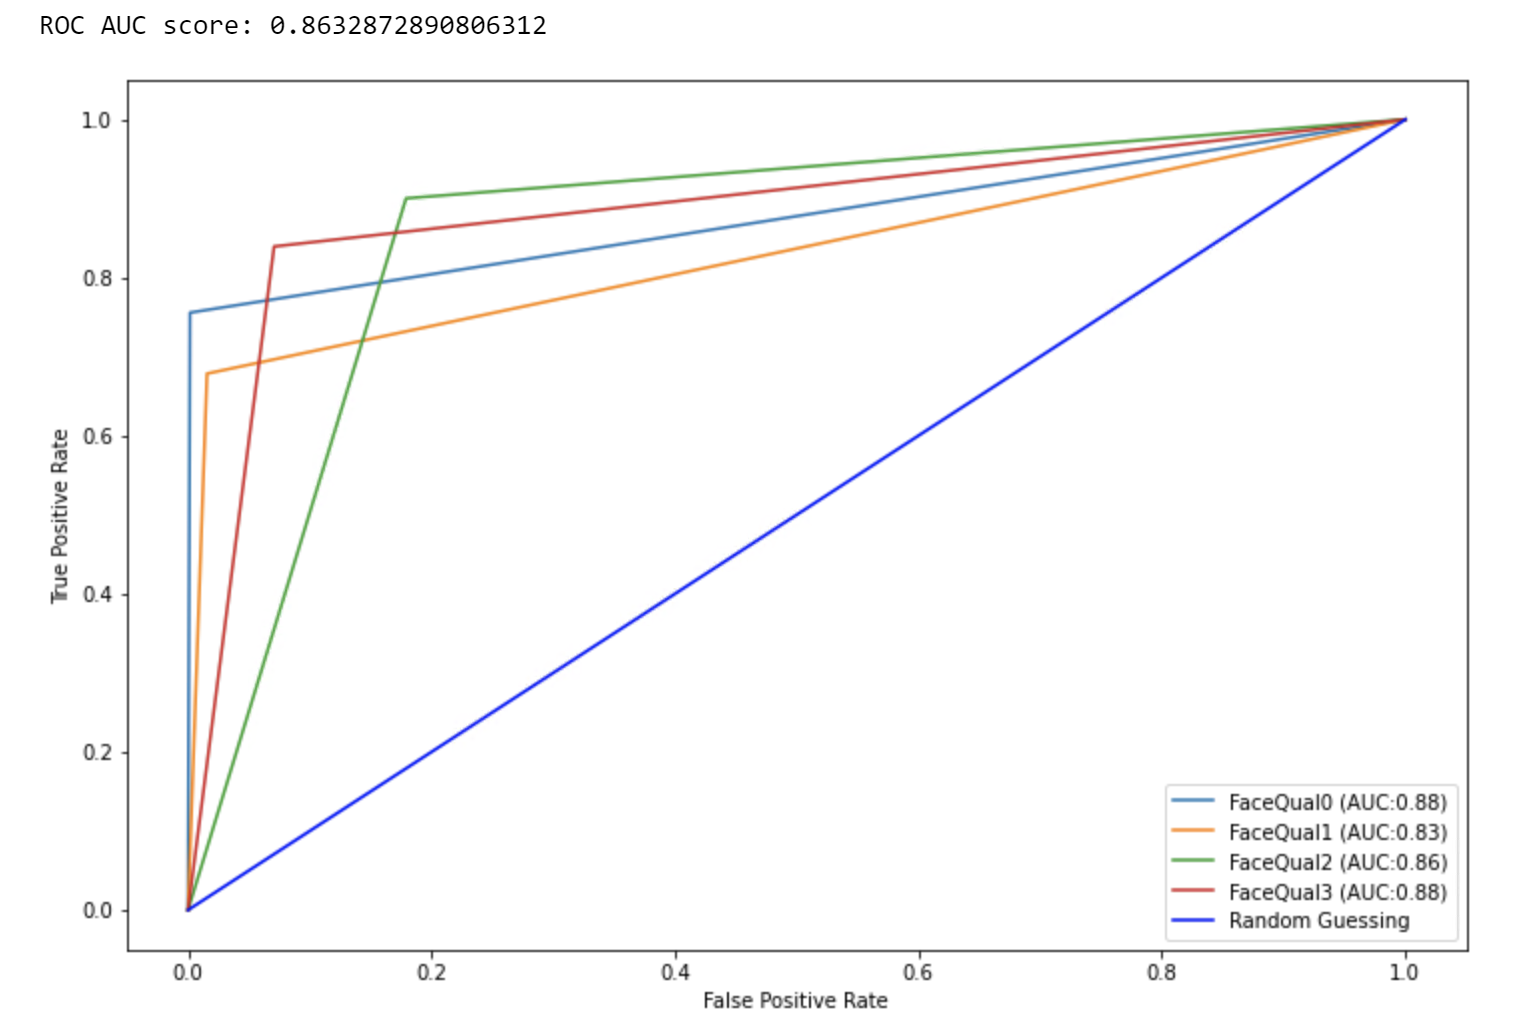
\includegraphics[width=150]{imgs/qualité/cr2/vgg16_111_roc.png}
\end{center}


\end{document}
